\documentclass[../seminar.tex]{subfiles}
\begin{comment}


\documentclass{ferseminar}
\usepackage{subfiles}
\usepackage[bottom]{footmisc}
\usepackage{graphicx}
\usepackage{caption}
\usepackage{subcaption}
\graphicspath{{../Slike/}}
\end{comment}

\begin{document}


Ostvarenje računalnog vida pomoću uparenih kamera (stereo sustava kamera) zahtijeva dva pripremna koraka:
\begin{itemize}
\setlength\itemsep{0.5em}
\item \textbf{Kalibracija stereo sustava} koja uključuje određivanje unutrašnje orijentacije i relativne orijentacije korištenih kamera
\item \textbf{Rektifikacija para slika} dobivenih stereo sustavom kako bi se dobile epipolarne slike čime se pojednostavljuje povezivanje točaka slika
\end{itemize}

Prije geometrijske kalibracije stereo sustava kamera s ribljim okom potrebno je odrediti matematički model kojim se opisuje projekcija 3D točaka na 2D sliku. Jedan način je proširiti perspektivni model \textit{pinhole} kamere s dodatnim uvjetima kako bi se obuhvatio efekt ribljeg oka na ravnini slike. Ovakav model je limitiran kutom vidnog polja koji je značajno ispod 180°. Osim toga, postoji mogućnost numeričke nestabilnosti prilikom kalibracije zbog nehomogene pokrivenosti virtualne ravnine slike. Zbog navedenog je bolje koristiti specijalni model ribljeg oka\cite{Abraham} koji se sastoji od dva koraka: idealno preslikavanje sfere slike u ravninu slike i subsekventna korekcija (engl. \textit{subsequent correction}).


\subsection{Vanjska i relativna orijentacija}

Prvi korak modeliranja ribljeg oka je određivanje mapiranja sfere pogleda u ravninu slike. Projekcija ribljeg oka
s vidnim poljem većim od 180° zahtijeva nelinearne transformacije zajedno s projekcijskom geometrijom. Kao i u slučaju modela jedne kamere projekcija 3D-točke scene (svijeta, engl. \textit{world}) s koordinatama $\boldsymbol{X}_W = (X_W,Y_W,Z_W)^T$ u točku slike 
$\boldsymbol{x'}_j = (x'_j,y'_j)$ se modelira kao niz transformacija koordinata koje sadrže ekstrinsične i intrinsične parametre kamere.  


Vanjska orijentacija (engl. \textit{exterior orientation}) stereo sustava kamera opisuje transformaciju koordinata 3D točke scene $\boldsymbol{X}_W$ u koordinate kamere $\boldsymbol{X}_{CL}$ lijeve kamere koristeći matricu rotacije $\boldsymbol{R}_{W,CL}$
i translacijski vektor $\boldsymbol{t}_{W,CL}$ kao ekstrinsične parametre.

\begin{equation}
\label{eq:eq_ext_ori1}
\boldsymbol{X}_{CL} = \boldsymbol{R}_{W,CL}(\boldsymbol{X}_W - \boldsymbol{t}_{W,CL})
\end{equation}

\hfill\break
\hfill\break
\hfill\break
\indent Relativna orijentacija opisuje transformaciju koordinata iz koordinatnog sustava lijeve kamere u k.o. desne kamere koristeći matricu rotacije $\boldsymbol{R}_{CL,CR}$ i translacijski vektor $\boldsymbol{t}_{CL,CR}$.

\begin{equation}
\label{eq:eq_ext_ori1}
\boldsymbol{X}_{CR} = \boldsymbol{R}_{CL,CR}(\boldsymbol{X}_{CL} - \boldsymbol{t}_{CL,CR})
\end{equation}

\begin{figure*}[ht!]
  \centering
    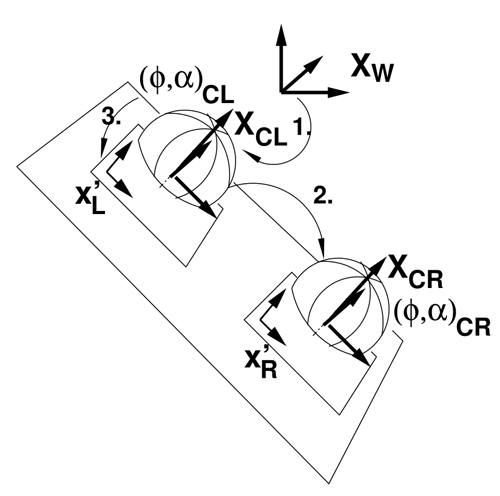
\includegraphics[width=.5\textwidth]{exterior_orientation.png}
   \caption{Koordinatni sustav i transformacije za stereo model kamera s ribljim okom (izvor: \cite{Abraham})}
  \label{fig:exterior_orientation}
\end{figure*}


\subsection{Epipolarna rektifikacija stereo sustava kamera s ribljim okom}


Epipolarna rektifikacija slika je geometrijska transformacija para slika u par slika s posebnim svojstvom: svaka točka scene $\boldsymbol{X}_i$ je projicirana u obje slike u istom retku ($y'_{L_i} = y'_{R_i}$). Time se pretraga za drugom točkom iz para točaka svodi na 1-D pretragu po retku slika.

\begin{figure*}[ht!]
  \centering
    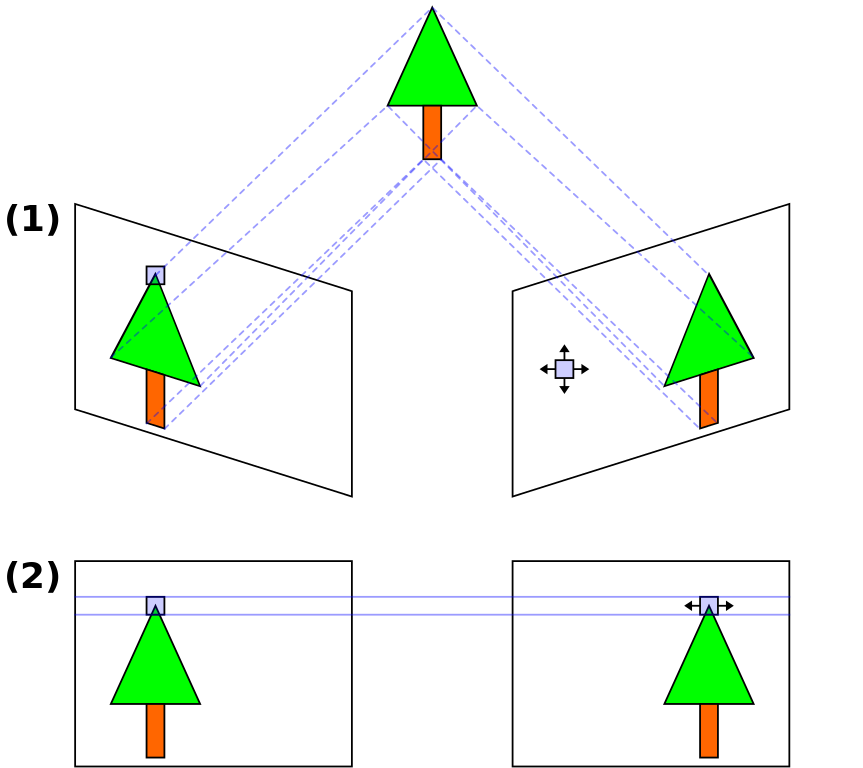
\includegraphics[width=.5\textwidth]{img_007_rectification01.png}
   \caption{Koncept rektifikacije stereo slika: prije (1) i poslije (2) rektifikacije (izvor: \cite{Wikipedia:Rectification})}
  \label{fig:rectification_idea}
\end{figure*}

Proces rektifikacije slika se može opisati kao reprojekcija 3D svijeta u virtualnu stereo kameru (engl. \textit{virtual stereo camera}). Virtualna kamera ima idealna svojstva: paralelne optičke osi, identične unutrašnje orijentacije (intrinsične parametre) i izostanak izobličenja. Projekcijski centri stvarne i virtualne stereo kamere se nalaze na istoj lokaciji (Slika \ref{fig:rectification_projection_centers}).

\begin{figure*}[ht!]
  \centering
    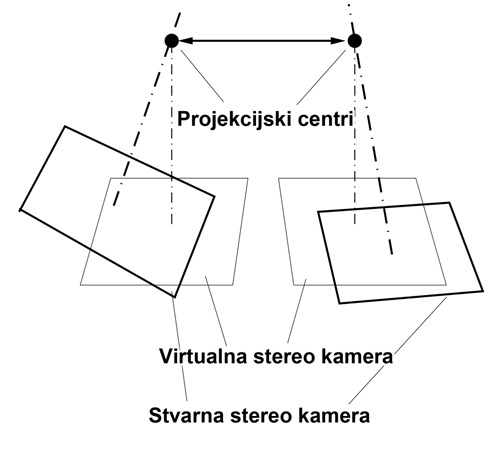
\includegraphics[width=.5\textwidth]{img_008_projection_centers_smaller.png}
   \caption{Stvarna i virtualna stereo kamera (izvor: \cite{Abraham})}
  \label{fig:rectification_projection_centers}
\end{figure*}


Koncept virtualne kamere ima svoje prednosti i nedostatke. Rektificirane slike su nezavisne od stvarne projekcije, virtualna kamera se može dizajnirati za paralelne epipolarne linije, računalni proces obrade slike ne mora poznavati svojstva stvarne kamere i može se dobro prilagoditi projekcijskom modelu virtualne kamere.
U prethodnom poglavlju su opisani modeli nelinearne projekcije ribljeg oka na ravninu slike no njihovim korištenjem se ne dobivaju epipolarne slike, epipolarne linije su krivulje. Zato se i komplicira pretraga odgovarajućih točaka u uparenim slikama što se može dobro vidjeti na jednostavnom primjeru u Slici \ref{fig:rectification_object_projection}. 

\begin{figure*}[ht!]
  \centering
    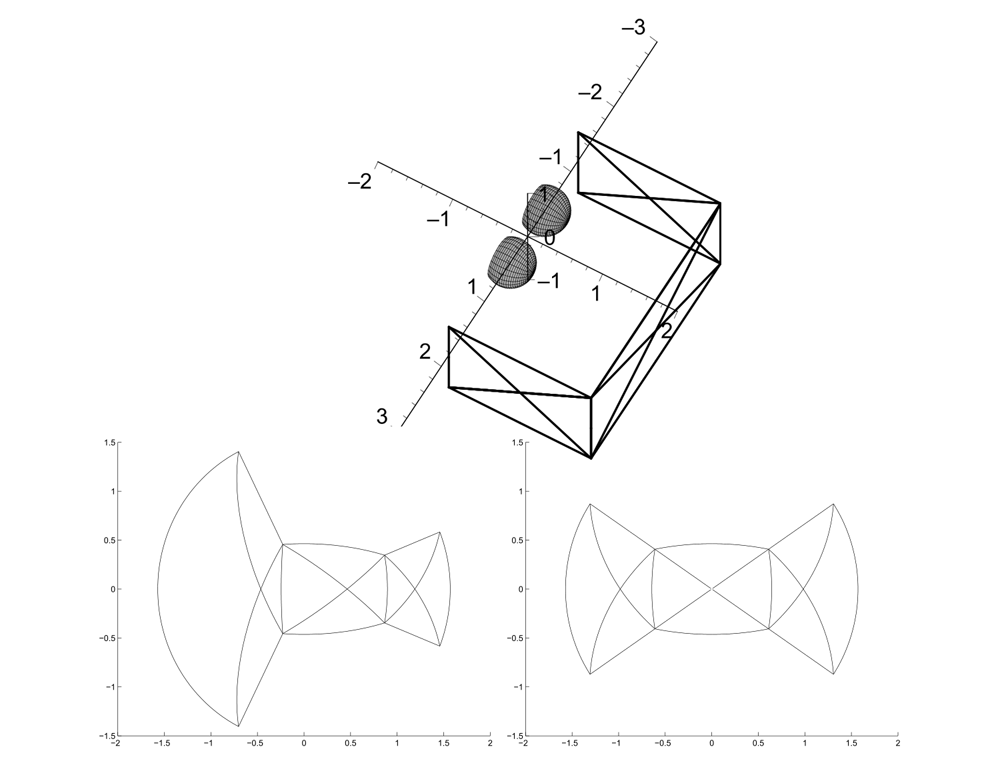
\includegraphics[width=.99\textwidth]{img_009_object_projection_medium.png}
   \caption{3D objekt, par kamera koje ga snimaju (riblje oko je prikazano kao sfera) i projekcije koje stvaraju (izvor: \cite{Abraham})}
  \label{fig:rectification_object_projection}
\end{figure*}


Poznavajući osnovna svojstva epipolarne geometrije moguće je definirati shemu rektifikacije za kamere s ribljim okom. 
U stereo sustavu kamera s dva projekcijska centra sve epipolarne ravnine sijeku jedna drugu pod određenim kutom (Slika \ref{fig:epipolar_planes}). 
Svaka ravnina je tako karakterizirana s nagibom (engl. \textit{pitch angle}) $\beta$. 
Kako bi se dobile paralelne epipolarne linije svaki redak rektificiranih slika mora odgovarati epipolarnoj ravnini. 
Razumijevanjem uzroka izobličenja odnosno modela stvaranja slike u kamerama s ribljim okom moguće je navedeno izobličenje ispraviti. 
Neka su $\beta = arctan(Y_V/Z_V)$, $\psi = arctan(X_V/\sqrt{Y^2_V+Z^2_V})$. Tada vrijedi model rektifikacije koji se tvori pomoću projekcijskih funkcija:
\begin{equation}
\label{eq:eq_projection_function_y}
y^* = r_{y^*}(\beta)
\end{equation}
\begin{equation}
\label{eq:eq_projection_function_x}
x^* = r_{x^*}(\psi)
\end{equation}

Projekcijskom funkcijom $y^*$ (\ref{eq:eq_projection_function_y}) se dobiva projekcija epipolarnih ravnina na retke rektificiranih slika. Projekcijska funkcija $x^*$ (\ref{eq:eq_projection_function_x}) definira projekciju unutar epipolarnih ravnina. 


\begin{figure*}[ht!]
  \centering
    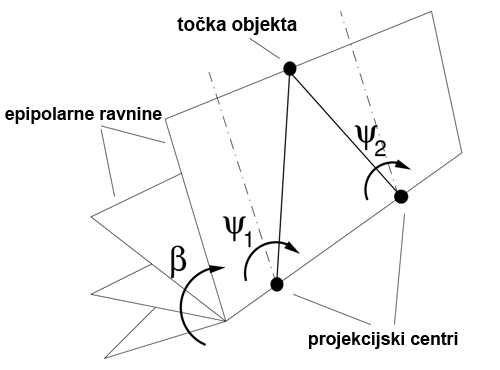
\includegraphics[width=.5\textwidth]{img_010_epipolar_planes_smaller.png}
   \caption{Epipolarne ravnine (pod kutom $\beta$) i projekcije (pod kutom $\psi$ unutar ravnina) (izvor: \cite{Abraham})}
  \label{fig:epipolar_planes}
\end{figure*}


Model rektifikacije za virtualnu kameru, definiran pomoću (\ref{eq:eq_projection_function_y}) i (\ref{eq:eq_projection_function_x}), se zapisuje kao $\boldsymbol{x'}_V = \boldsymbol{T}_V (\boldsymbol{q}_V)$ ($V$ je znak virtualne kamere).\cite{Abraham}
 
Model $\boldsymbol{T}_V$ je nelinearna funkcija koja transformira koordinatu $\boldsymbol{q}_V = (X_v,Y_v,Z_v)$ iz koordinatnog sustava kamere u k.s. slike virtualne kamere $\boldsymbol{x'}_V = (x'_v,y'_v)$, vrijedi sljedeće:

\begin{equation}
\label{eq:eq_rectification_model_y}
y'_V = c_{yV} · r_{y^*}(\beta) + y_{HV}
\end{equation}

\begin{equation}
\label{eq:eq_rectification_model_x}
x'_V = c_{xV} · r_{x^*}(\psi) + x_{HV}
\end{equation}

Funkcije $r_{x*}$ i $r_{y^*}$ mogu biti različite. Primjerice, kombinacija $r_{x*} = \tan[\psi]$ i $r_{y^*} = \beta$ daje cilindričnu rektifikaciju koja minimizira izobličenje\cite{RoyMeunierCox}.

Pomoću kalibracijskog modela stvarne kamere (Slika \ref{fig:calibration_board}) i rektifikacijskog modela virtualne kamere (\ref{eq:eq_rectification_model_y} i \ref{eq:eq_rectification_model_x}) transformacija iz koordinata virtualne kamere u koordinate stvarne slike se zapisuje na sljedeći način:

\begin{equation}
\label{eq:eq_transformation}
\boldsymbol{x'} = \boldsymbol{T}(R_{C,V}\boldsymbol{T}^{-1}_V(\boldsymbol{x'}_V))
\end{equation}

Rotacijska matrica $R_{C,V}$ definira rotaciju između koordinatnih sustava stvarne i virtualne kamere. Ona ovisi o relativnoj orijentaciji stereo kamera.

Koncept virtualne kamere kombiniran s različitim projekcijskim funkcijama za proces rektifikacije omogućuje rektifikaciju slika s vidnim poljem većim od 180° u horizontalnom i vertikalnom smjeru.
Rektifikacijski model se može odabrati prema potrebi. U nastavku su dva primjera:
\begin{itemize}
\setlength\itemsep{2em}
\item Epipolarni ekvidistantni rektifikacijski model
\item Epipolarna stereografska rektifikacija
\end{itemize}

\subsubsection{Epipolarni ekvidistantni rektifikacijski model}

Na temelju geometrije epipolarnih ravnina (Slika \ref{fig:epipolar_planes}) i ekvidistantnog projekcijskog modela transformacija koordinata kamere $\boldsymbol{X}_C$ 
u koordinate slike $\boldsymbol{x'}$ se izvodi na sljedeći način. Neka su $\psi = arctan(\frac{X}{\sqrt{Y^2 + Z^2}})$ i $\beta = arctan(\frac{Y}{Z})$.
Tada vrijedi sljedeće:

\begin{equation}
\label{eq:eq_transformation_equidistance_x}
x' = c_x\psi + x'_H
\end{equation}

\begin{equation}
\label{eq:eq_transformation_equidistance_y}
y' = c_y\beta + y'_H
\end{equation}

Koordinata $y'$ ovisi samo o kutu $\beta$, a koordinata $x'$ ovisi o lokaciji točke u epipolarnoj ravnini. Kutovi $\beta$ i $\psi$ su projicirani u ekvidistantnim koracima u sliku pa se vrijednosti $y'_H$ i $x'_H$ mogu praktički zanemariti.
Neka su $x^*$ i $y^*$ normalizirane koordinate slike (\ref{eq:eq_projection_function_x} i \ref{eq:eq_projection_function_y}). 
Tada vrijedi inverzna transformacija iz koordinata slike $\boldsymbol{x'}$ u koordinate kamere $\boldsymbol{X}$:

\begin{equation}
\label{eq:eq_transformation_camera}
\begin{pmatrix} X \\ Y \\ Z \end{pmatrix} = \begin{pmatrix} \sin x^* \\ \cos x^* \sin y^* \\ \cos x^* \cos y^* \end{pmatrix}
\end{equation}

Slika \ref{fig:rectification_object_projection_epipolar_equidistant} prikazuje rektifikaciju pomoću epipolarnog ekvidistantnog rektifikacijskog modela (engl. \textit{epipolar-equi-distant rectification model}).

\begin{figure*}[ht!]
  \centering
    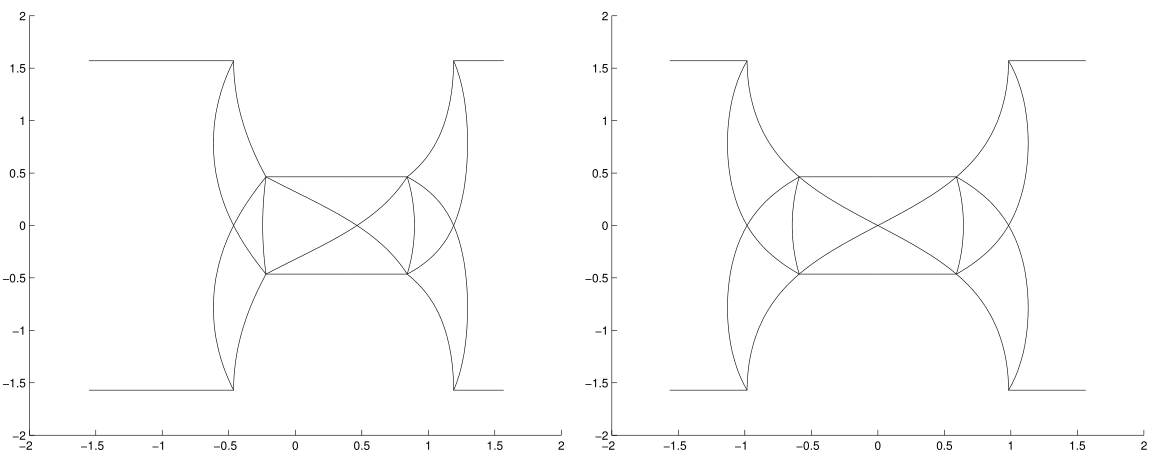
\includegraphics[width=.99\textwidth]{img_011_epipolar_equidistant.png}
   \caption{Projekcija pomoću epipolarnog ekvidistantnog rektifikacijskog modela (istog objekta kao u Slici \ref{fig:rectification_object_projection}) (izvor: \cite{Abraham})}
  \label{fig:rectification_object_projection_epipolar_equidistant}
\end{figure*}

\subsubsection{Epipolarna stereografska rektifikacija}

Navedene transformacije (\ref{eq:eq_transformation_equidistance_x}, \ref{eq:eq_transformation_equidistance_y} i \ref{eq:eq_transformation_camera}) zahtijevaju računanje trigonometrijskih funkcija. Za procesiranje u stvarnom vremenu to predstavlja problem zbog brzine izvođenja. U epipolarnoj stereografskoj rektikaciji (engl. \textit{epipolar stereographic rectification}) koristi se drugi set jednadžbi transformacija:


\begin{equation}
\label{eq:epipolar_stereographic_x}
x' = c·\frac{X}{\sqrt{X^2+Y^2+Z^2} + \sqrt{Y^2+Z^2}} + x'_H
\end{equation}

\begin{equation}
\label{eq:epipolar_stereographic_y}
y' = c·\frac{Y}{\sqrt{Y^2+Z^2} + Z} + y'_H
\end{equation}

Iz normalizirane slike u koordinate kamere:

\begin{equation}
\label{eq:eq_transformation_camera}
\begin{pmatrix} X \\ Y \\ Z \end{pmatrix} = \begin{pmatrix} \frac{2x^*}{1+{x^*}^2} \\ \frac{1-{x^*}^2}{1+{x^*}^2}\frac{2{y^*}^2}{1+{y^*}^2} \\ \frac{1-{x^*}^2}{1+{x^*}^2}\frac{1-{y^*}^2}{1+{y^*}^2} \end{pmatrix}
\end{equation}




Koristeći jedan od navedenih modela rektifikacije omogućena je brza stereo pretraga odgovarajućih točaka na slikama.
Pretraga se može ubrzati koristeći tablice s predizračunatim vrijednostima. Dostupno je vidno polje veće od 180°, izuzetak su polovi slika gdje nema stereo informacije.








\end{document}
